\documentclass{frontiersSCNS} 
\usepackage{url,hyperref,lineno,microtype,subcaption}
\usepackage[onehalfspacing]{setspace}
\linenumbers


\def\keyFont{\fontsize{8}{11}\helveticabold }
\def\firstAuthorLast{Marion {et~al.}} 
\def\Authors{Zachary H. Marion\,$^{1,*}$ and Christopher A. Hamm\,$^{2}$}
\def\Address{$^{1}$Department of Ecology \& Evolutionary Biology, University of Tennessee, Knoxville, TN, USA \\

$^{2}$Department of Ecology \& Evolutionary Biology, University of Kansas, Lawrence, KA, USA  }
\def\corrAuthor{Zachary H. Marion}
\def\corrEmail{zmarion@vols.utk.edu}

%%%%%%
%%%%%%
%%%%%%

\begin{document}
\onecolumn
\firstpage{1}

\title[Endosymbiont infection estimation]{A hierarchical Bayesian approach to estimate endosymbiont infection rates} 

\author[\firstAuthorLast ]{\Authors} %This field will be automatically populated
\address{} %This field will be automatically populated
\correspondance{} %This field will be automatically populated

\extraAuth{Department of Ecology \& Evolutionary Biology, University of Tennessee, 569 Dabney Hall, 1416 Circle Drive, Knoxville, TN, 37996, USA}

\maketitle
\begin{abstract}

\section{}
Endosymbionts may play an important role in the evolution of the Insecta. Bacteria such as \emph{Wolbachia, Cardinium, \emph{and} Rickettsia} are known to manipulate their host' reproduction to facilitate their own. Indeed, there are many well know cases where \emph{Wolbachia} (Alphaproteobacteria: Rickettsiaceae
) induces one of four manipulative phenotypes (cytoplasmic incompatibility, male killing, feminization, and parthenogenesis). The scale of infection among species has been a major subject of investigation, but this is not an easy endeavor and different approaches have yielded different estimates. One aspect of this problem that may be underappreciated arises when multiple yet independent samples are taken within a species. When independent samples within species are treated as levels of a hierarchy the problem is greatly simplified because error propagates through the model in a realistic and intuitive manner. Here, we present a hierarchical Bayesian approach to estimate infection frequency where multiple independent samples were collected across multiple taxonomic levels. We apply this model to estimate the rates of infection for \emph{Wolbachia} in the Lepidoptera, and apply the model with a correction to account for phylogenetic non-independence. In addition, we highlight the present body of knowledge regarding \emph{Wolbachia} and its effects with regards to the Lepidoptera. Our model estimates suggests that the rate of endosymbiont infection in the Lepidoptera is lower than previously estimated. Given our limited knowledge regarding the phenotypes induced by these endosymbionts, we urge caution when interpreting the results of a positive assays.

\tiny
 \keyFont{ \section{Keywords:} \emph{Wolbachia}, Lepidoptera, modeling, keyword, kewyord} % keywords should not be present in the title 
\end{abstract}

\section{Introduction}

Bacterial endosymbionts have been known to inhabit insects for decades. These endosymbionts are maternally transmitted through the cytoplasm of the egg. \textit{Wolbachia} was the first of these endosymbionts to be discovered when \citet{Hertig:1924wy} examined the adult ovaries and testes of \textit{Culex pipiens} (hence the specific epithet \textit{Wolbachia pipientis}) \citet{Hertig:1936}. Some years later, \citet{Yen:1971tc} observed that male \textit{C. pipiens} from one geographic area may not successfully reproduce with females from a different area, and reciprocal crosses could produce similar results; this phenomenon was given the name \textit{cytoplasmic incompatibility}. A \textit{Rickettsia}-like organism was determined to be the causative agent, which was later determined to be \textit{Wolbachia} \citep{Yen:1973vx}.

Contemporary researchers detect the presence of \textit{Wolbachia} via the polymerase chain reaction (PCR). Today, any sample can be screened in a quick, easy, and relatively inexpensive manner \citep{Baldo:2006p7025,Simoes:2011p11073}, however, this development is relatively recent. Prior to the advent of PCR, \textit{Wolbachia} infection was only confirmed through painstaking work that included electron microscopy and other microbiological techniques. Indeed, these methods required such effort that they were employed once a researcher had an \textit{a priori} reason suspect the presence of the bacterium; we are aware of no cases in which exploratory assays for \textit{Wolbachia} were conducted prior to the appearance of PCR. It was under these circumstances that a researcher would observe a likely reproductive manipulation phenotype (\emph{male killing, feminization, \emph{or} parthenogenesis}) and then attribute it to \textit{Wolbachia}.

Careful laboratory work is required to determine what phenotype (if any) is induced by an endosymbiont. With the arrival of PCR and Sanger sequencing it became feasible to conduct exploratory investigations for the presence of \textit{Wolbachia}, though few studies conducted the experimental work to determine if any reproductive manipulation was occurring. The effects of \textit{Wolbachia} infection are complex and depend on an interaction between the genomes of the endosymbiont and the host. For example, the phenotypic effects of one strain of \textit{Wolbachia} may be very different if moved into another host \citep{Rigaud:2001fv,Hoffmann:2011p11474}. Additionally, there may be extensive genomic differences between closely related strains of \textit{Wolbachia} \citep{Ishmael:2009p8257}. Though most famous for its status as a "reproductive parasite," \textit{Wolbachia} infections have been shown to induce no manipulation at all \citep{Hamm:2014cv,Zhang:2010jl,Zhang:2013eo}. Without careful experimentation, it is not scientific to assume that \textit{Wolbachia} will manipulate a host simply because of a positive PCR assay. 

The Lepidoptera (Arthropoda: Insecta) represent the best studied order of animals. Because of historic interest in their physical beauty and their contemporary economic importance the literature is replete with detailed knowledge regarding their distribution and life history. The  Lepidoptera is a large Order containing approximately 160,000 species in 124 families, which is approximately 13\% all species currently known \cite{Regier:2013fp}. In addition to research focused on the Lepidoptera for pure biological reasons, the Lepidoptera are also well represented on lists of endangered or threatened species \citep{Hamm:2014wi}. Researchers have tended to focus on certain groups of Lepidoptera, such as the butterflies (e.g. Nymphalidae, Lycaenidae and Pieridae) or groups of economically important pest species such as the Crambidae (which contains the Asiatic rice borer \textit{Chilo suppressalis} and Noctuidae (which contains the armyworms of the genus \textit{Spodoptera}); this results in a bias towards certain groups and leaves most of the remaining families understudied. 

Experiments to determine if a manipulative phenotype exits have been conducted for six species of Lepidoptera and report that \emph{cytoplasmic incompatibility, male killing, \emph{and} feminization} occur (Table 1). We note that the report of \textit{male killing} in \textit{Ephestia kuhniella} is a result of \textit{Wolbachia} transfected from \textit{Ostrinia scapulalis}. Because of the high level of interest in Lepidoptera research, there is a considered enthusiasm for investigating the role that \textit{Wolbachia} has played in its evolution. A vital first step towards this goal is the estimation of \textit{Wolbachia} infection rates in the Lepidoptera. 

ZACH, I'LL NEED TO YOU SET THE LAST PARAGRAPH OF THE INTRO. I CAN'T WRITE ABOUT IT WELL BUT MY ABORTED ATTEMPTS ARE BELOW.

Here, we develop and employ a novel approach to the estimation of \textit{Wolbachia} infection frequencies across the Lepidoptera. Our model explicitly accounts for issues that arise with real world data, such as those relating to estimating infection levels at different scales. For example, there may be multiple observations of infection frequency collected from different populations within a species, often with disparate sample sizes. We do not consider it appropriate for these samples to be completely pooled, as that ignores population differences in infection frequency. Nor should observations within species be considered independent, because of shared ancestry.  Similarly, there may be single samples collected from many different species within a family. In this case, individual sampling error should be accounted for when estimating family level infection rates. Finally, we consider that there has been a bias towards studying only a few families of the Lepidoptera. This uneven sampling can cause a few well-studied families to drive estimates of overall infection frequency. Each of these concerns can be specifically considered and accounted for with hierarchical Bayesian approaches that explicitly incorporate phylogenetic correlations. 


\section{Materials \& Methods}
\subsection{Motivating data and previous analyses}

 Both \cite{Weinert:2015aa} and \cite{Ahmed:2015aa} used a likelihood-based approach to describe the distribution of \emph{Wolbachia} infection across arthropods and Lepidoptera, respectively. Both studies used beta-binomial models to estimate the mean proportion of individuals infected within a given species \citep{Hilgenboecker:2008aa}. They used the same distribution to calculate the incidence of infection as well, where incidence was the proportion of species infected above a threshold frequency $c$  \citep[i.e.,, one infection in 1000 individuals, or 0.001;][]{Weinert:2015aa}. 

In the case of \textit{Wolbachia}, insects screened for this bacterium may either be positive or not positive. It is important to state that ?not positive? is the appropriate state here because an infection could have been missed for a number of reasons, including low density infections \citep{Schneider:2014jv}. However, for the sake of simplicity, we will treat \textit{Wolbachia} infection status as two mutually exclusive outcomes, (0 or 1; positive or not positive). This makes the question of infection a binomial sampling problem. The issue is the way that likelihood deals with error at each level, or rather how it does not. We will demonstrate this problem with two examples. First, let us assume that 200 individuals of a species are assayed for \textit{Wolbachia}, and 100 of those tests are positive for infection. The mean estimate of infection is 0.5 and the 95\% exact binomial confidence interval is 0.43 ? 0.57. Next, let us say that two individuals from a species were assayed for \textit{Wolbachia}, and one tested positive. For this example, the proportion infected in this species is 0.5, however, the 95\% confidence interval is 0.01 ? 0.99. It is clear that there is uncertainty around each estimate and that uncertainty varies with sample size. For this error to be properly incorporated into any estimate it must be treated at each level of the analysis (each species), rather than at the level of the study. 

\subsection{Data}
We used the data set synthesized by \citet{Weinert:2015aa}, which contains records from thousands of individual sampling efforts across the Arthropoda.  These data were arranged such that each row represented one independent sampling event (though each row may contain multiple individuals) and contained information on the family, genus, species, endosymbiont genus, number of individuals assayed, and number of positive individuals. We filtered these data such that they contained only \textit{Wolbachia} assays of Lepidoptera. The filtered data set contained 1037 sampling events on 10860 individual Lepidoptera, of which 3607 screened positive for \textit{Wolbachia} infection. We imported these data into the program R v3.2 (R Core Development Team) and there conducted all subsequent analyses. All data and code necessary to reproduce the analyses and figures in this paper are freely available on FigShare (DOI TBD: \textit{NB}, the data will be accessioned to FigShare once the manuscript and code are in their final form).

To correct for any influence of the relatedness among families in our analysis, we used the Lepidoptera phylogeny of \citet{Regier:2013fp}, which contained 115 of the 124 families in the order. The tree was pruned to remove duplicate families and those not present in the  \cite{Weinert:2015aa} dataset. We then made the tree ultrametric following the penalized likelihood method of \citet{Sanderson:2002vy} using tools in the \textit{ape} package \citep{Paradis:2004dv}. To incorporate phylogenetic history into the Bayesian model, we used the pruned ultrametric tree to create a series of phylogenetic correlation matrices. We constructed one matrix in which we assumed that \textit{Wolbachia} infection status was distributed according to Brownian Motion (BM), a model of trait evolution that assumes neighboring taxa share that trait due to common ancestry \citep{Paradis:2012wn}. We also constructed matrices that assumed trait evolution followed an Ornstein-Uhlenbeck (OU) process, which places constraints around which a character evolves \citep{Paradis:2012wn}. Relative to the BM, the OU model has two additional parameters: $\theta$ (the "optimal" value for a character), and $\alpha$ (the rate at which $\theta$ moves towards $\alpha$) \citep{Paradis:2012wn}. The $\alpha$ value can range from 0 - 1; When $\alpha$ is 0 the model is effectively pure BM and becomes less so as $\alpha$ increases. We rescaled the Phylogeny using three alpha values to examine their impact: $\alpha$ = 0.1 (similar to BM), $\alpha$ = 0.5, and $\alpha$ = 0.9 (very different than BM).

\subsection{Bayesian hierarchical models}
	In contrast to \cite{Ahmed:2015aa}, we adopted a hierarchical Bayesian approach to estimate the probability of infection prevalence within and among species of Lepidoptera using a subset of the data from \cite{Weinert:2015aa}. Each observation ($N=1037$)---the number of \emph{Wolbachia}-infected individuals---was nested within species ($S=419$) and  modeled as:

\begin{equation}
	infected_{i,j} \sim \mathrm{Binomial}(n_{i}, \theta_{j}).
\end{equation}

where $i = 1, 2, \ldots, 1037$ and $j = 1, 2, \ldots, 419$. Here $infected_{i,j}$ indicates the number of infected individuals from the $i$th observation of the $j$th species,  $n_{i}$ is the total number of screened insects in observation $i$, and $\theta_{j}$ is the probability of infection for species $j$. 

	We then assumed the species-level probabilities of infection were normally-distributed with family-level means ($\mu_{k}$) and standard deviations ($\sigma_{k}$) where $k = 1, 2, \ldots, 28$ families. For computational efficiency, we used a non-centered parameterization of the normal \citep{Papaspiliopoulos:2007aa}. The normal distribution is unconstrained, but $\mathbf{\theta}$ is bounded between zero and one. Therefore the species-level $\theta$s were logit transformed such that  

	\begin{equation}    
		\mathrm{logit} (\theta_{j}) \sim \mathrm{Normal}(\mu_{k}, \sigma_{k}).
	\end{equation}
The mean ($\mu_{k}$) describes the average probability of infection within a lepidopteran species family on the log-odds scale and can be back-transformed using the inverse-logit function. 

The standard deviation ($\sigma$) measures how much variation in the probability of infection there is across species. If $\sigma$ is small, then infection probabilities will be similar among species. Conversely, if $\sigma$ is large, species-specific probabilities of infection will be more idiosyncratic. Data sparsity can be a problem in hierarchical models, especially for the estimation of scale parameters like variances. Because there were several species with few observations, we used a shrinkage prior \citep{Carvalho:2009aa,Carvalho:2010aa}
for the species-specific $\sigma$s: 
	\begin{align}
		\sigma_{k} 	&= 	 	t_{\nu}^{+}(0,\tau) \nonumber \\
        \tau		&\sim	t_{\nu}^{+}(0,1)     
	\end{align}

where $t_{3}^{+}$ is half-Student-t distribution with $\nu=3$ degrees of freedom. 

We modeled $\mu$, the vector of log-odds infection probabilities for families using a multivariate normal distribution:

\begin{equation}
	\begin{bmatrix}
		\mu_{1} \\
        \mu_{2} \\
        \vdots \\
        \mu_{k}
	\end{bmatrix}
    = 
    \textrm{MVNormal}(\gamma, \Sigma).
\end{equation}
with the mean log-odds probability of infection across Lepidoptera ($\gamma$) and covariance matrix $\Sigma$. To account for phylogenetic non-independence among families, we constructed sigma as:

\begin{equation}
	\Sigma = \boldsymbol{\eta} \;	\boldsymbol{\Omega} \; \boldsymbol{\eta}
\end{equation}

where $\boldsymbol{\eta}$ is a $k \times k$ diagonal matrix with the overall standard deviation on the diagonals and $\boldsymbol{\Omega}$ is a $k \times k$ phylogenetic correlation matrix. We then put regularizing priors on both $\gamma$ and $\eta$:

\begin{align}
	\gamma 	&\sim \mathrm{Normal}(0, 5) \nonumber \\
	\eta   	&\sim t_{\nu}^{+}(0,5)
\end{align}

where again $t_{3}^{+}$ is half-Student-t distribution with $\nu=3$ degrees of freedom. 

Posterior probabilities for model parameters were estimated using Markov chain Monte Carlo (MCMC) sampling in the Stan programming language \citep{Carpenter:2016aa} via the RStan interface \citep{stan:2016aa}. For each model, four MCMC chains were used with 5,000 iterations each. The first 2,500 iterations for each chain were adaptive and thus discarded as warm-up. We used several diagnostic tests to confirm that each model had reached a stationary distribution including visual examination of MCMC chain history and calculation of effective sample size (ESS) and the Gelman and Rubin convergence diagnostic \citep{Gelman:1992aa,Brooks:1998aa}. In particular, model convergence was assessed by inspecting the diagnostics of the log-posterior density. 

We used WAIC \citep[the widely applicable or Watanabe-Akaike information criterion;][]{Watanabe:2010aa,Gelman:2014aa} to compare models with different phylogenetic correlation matrices (e.g., Brownian motion vs. OU processes) using functions in the loo package \citep{Vehtari:2016aa}. 

\section{Results}
After filtering the \citet{Weinert:2015aa} data to contain only Lepidoptera that were screened for \textit{Wolbachia} we retained 1037 independent sampling events of 411 unique species from 28 families, representing a total of 10860 individual assays. Of these, 3607 samples from 163 species and members of 19 families were scored PCR positive for \textit{Wolbachia}.

ZACH, please describe the model results (diagnostics, chain mixing, posterior predictive.

\begin{enumerate}  
\item WAIC scores among models
\item Median estimate for Order, almost identical regardless of model
\item Discuss family level estimate (is there a correlation between sample size and CI?)
\end{enumerate}


\section{Discussion}

Previous research on \textit{Wolbachia} in the Lepidoptera has estimated the infection frequency at very high levels, ~80\% \citet{Ahmed:2015aa} and ~77\% \citet{Weinert:2015aa}. 

Our model predicts that median \textit{Wolbachia} infection frequency in the Lepidoptera is significantly lower than previous studies have reported. 

It is interesting to consider that the median infection frequency estimates for the Lepidoptera do not significantly change when the model considers relatedness by incorporating phylogenetic information. Also, the WAIC scores did not significantly var

Whether we incorporate a phylogeny or not, use pure BM process or an OU with varying alpha values, we get the same answer. 



Seven species (out of >450 assayed) in four families of Lepidoptera have been assayed for a \textit{Wolbachia} induced phenotype. 

In many respects, scientific research with regards to \textit{Wolbachia} is still in its "natural history" phase, wherein we describe the distribution and effects of infection.  

Lower than \citet{Hilgenboecker:2008aa}
mean is near \citet{Ahmed:2015aa} and \citet{Weinert:2015aa}, but variance is much higher

Likely to be differences between male and female infection levels if there is an induced phenotype (indirect evidence). The data presented here pool males and females, which may bias the results.

Bias in sampling must be accounted for, make a plot of families we have within the Lepidoptera.

Given the potential use \textit{Wolbachia} as a potential biological control agent



It is a bit simplistic to just assume that there will be a reproductive manipulation \citep{Nice:2009p7399,Hamm:2014wi}. We strongly encourage that assays for endosymbionts be conducted prior to the translocation or interbreeding of insects of conservation concern and, if to conduct controlled matings as guided by the results of those assays. 

It could still be in the genome, (example from \textit{Drosophila} and \textit{Nasonia} REFS.

Don?t forget \citet{Prout:1994th}, which demonstrated that vertically transmitted reproductive \textit{Wolbachia} should evolve to minimize harm to the host. 



\citet{vanNieukerken:2011a123}

\citet{Jiggins:2001p7754}

\citet{Jiggins:2001uo}


Make point that Fem \& MK likely manipulate the piRNA - REF!

We conclude that the science of microbes in the Lepidoptera, especially with regards to the endosymbiont \textit{Wolbachia}, is still in its natural history phase wherein discovery is still largely in the descriptive phase, and as such we urge caution when interpreting positive \textit{Wolbachia} assays and extrapolating consequences. 

The standard Wolbachia paradigm holds that the endosymbiont is a reproductive parasite that manipulates its host?s reproduction to facilitate its own. The phenotypic effects of infection are known for only a handful of Lepidoptera, given the recent advances in \textit{Wolbachia} research in other taxa (particularly \textit{Drosophila}) which demonstrate that infection does necessarily result in reproductive manipulation, we urge caution when interpreting positive \textit{Wolbachia} assays and extrapolating consequences.

We present a new analysis estimating the infection frequency of \textit{Wolbachia} in the Lepidoptera, which contrasts with a recently published estimate. Our model treats error hierarchically, which we feel is appropriate given the structure of the data. 

Slow your ever-loving role ? which will translate into ?we urge caution.?
The model cited in \citet{Nice:2009p7399} make a lot of assumptions as to how \textit{Wolbachia} works, please note that they did not estimate a phenotype.
Wolbachia research in the Lepidoptera is still in the Natural History / Discovery phase

Indirect evidence - Look for signature of reproductive manipulation: biased sex ratios, mito ? nuclear discord in phylogenies. 


Model of \textit{Wolbachia} infection frequency - Handles error hierarchically (just like the data), consider binomial confidence interval for 1+ of 2. It?s huge! - Our model is awesome, generates credible intervals that are more reasonable - More like 50\% with HPD of 30 ? 60. Plot the posteriors. 


Some families only had one sample, in which case there was little information for the model and inferences for these groups were driven by the prior and had large CIs (\textbf{Figure 3}).

\newpage

%%%%%%
%%%%%%
%%%%%%

\section*{Conflict of Interest Statement}
The authors declare that the research was conducted in the absence of any commercial or financial relationships that could be construed as a potential conflict of interest.

%%%%%%
%%%%%%
%%%%%%

\section*{Author Contributions}
ZM and CH conceived of the experiment; ZM and CH conducted the analyses; ZM and CH wrote the manuscript. 

\section*{Funding}
The authors received no external funding to conduct this research.

\section*{Acknowledgments}
We wish to thank James Fordyce, Christopher Peterson, Brian O'Meara and Jeremy Beaulieu for their input and advice during the preparation of this manuscript.

\section*{Supplemental Data}
 \href{http://home.frontiersin.org/about/author-guidelines#SupplementaryMaterial}{Supplementary Material} should be uploaded separately on submission, if there are Supplementary Figures, please include the caption in the same file as the figure. LaTeX Supplementary Material templates can be found in the Frontiers LaTeX folder 
\newpage
\bibliographystyle{frontiersinSCNS_ENG_HUMS} 
\bibliography{Wolbachia}
\newpage 

%%%%%%
%%%%%%
%%%%%%

\section*{Figures}

\begin{figure}[h!]
\begin{center}
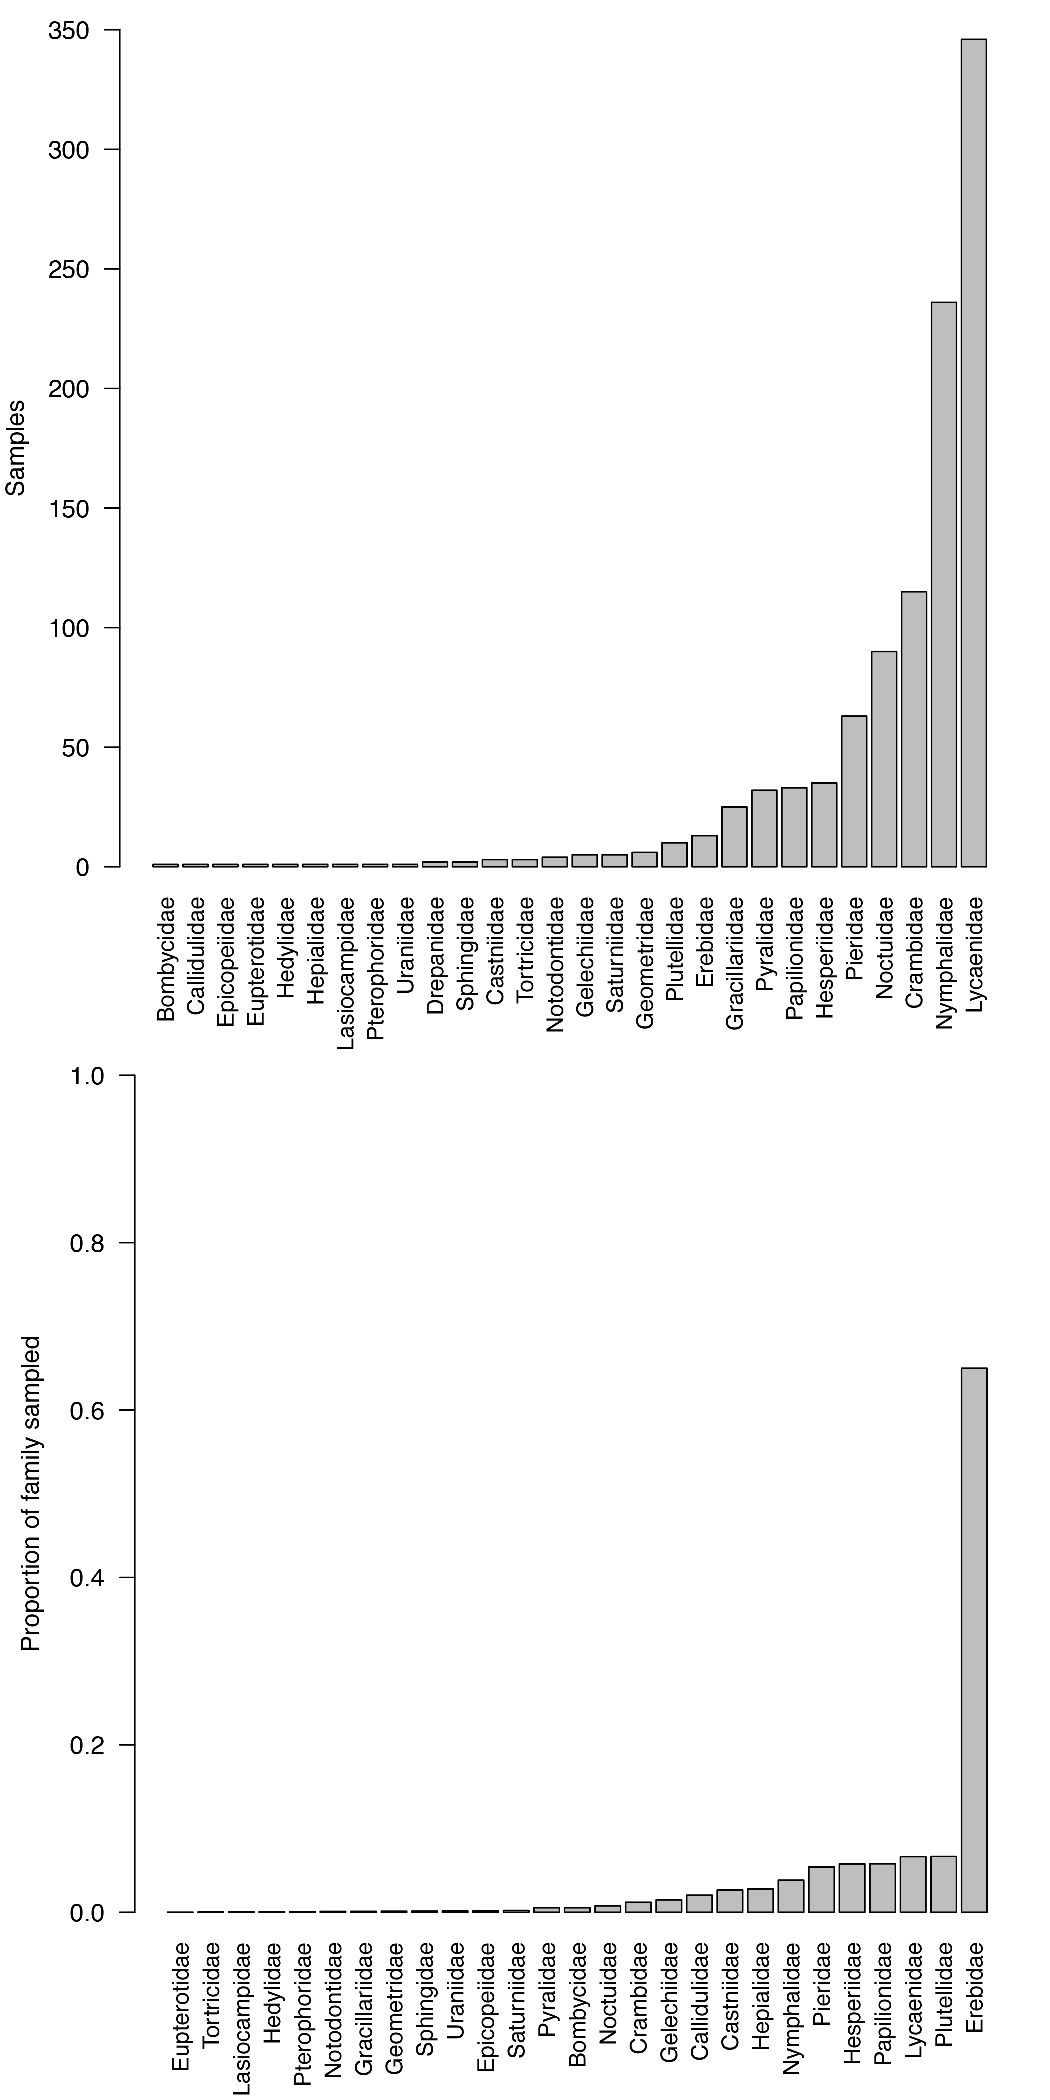
\includegraphics[width=85mm]{Fams_n_Props.pdf}% This is a *.jpg file
\end{center}
\caption{\textit{Wolbachia} sampling by family for total number \textbf{(A)} and scaled by proportion of species sampled in each family \textbf{(B)}.}
\label{histograms}
\end{figure}

\newpage

\begin{figure}[h!]
  \begin{center}
    \includegraphics[width=85mm]{infection_Prob.pdf}
    \caption{Posterior density plots for the average frequency of \textit{Wolbachia} infection across Lepidoptera. Each posterior estimate is jittered and superimposed on the violins with transparency. Fatter regions of the  violins indicate regions of higher posterior density, as do darker regions of jittered points. Horizontal bars indicate the median and upper and lower 95\% Highest Density Interval (HDI).  Models (L to R): NP = No Phylogenetic correction; BM = Brownian Motion; OU = Ornstein-Uhlenbeck with varying levels of $\alpha$ (0.1, 0.5, 0.9); Model Avg. = WAIC model weighted averaging.}
 \label{grand}
  \end{center}
\end{figure}

\newpage 

\begin{figure}[h!]
  \begin{center}
    \includegraphics[width=180mm]{familyplotAvg.pdf}
    \caption{Posterior density plots for the average frequency of \textit{Wolbachia} infection among 28 families of Lepidoptera. Each posterior estimate is jittered and superimposed on the violins with transparency. Fatter regions of the  violins indicate regions of higher posterior density, as do darker regions of jittered points. Horizontal bars indicate the median and upper and lower 95\% Highest Density Interval (HDI).}
 \label{familyplot}
  \end{center}
\end{figure}
\newpage

% I think the model averaging gives the appearance of tight CIs when they really don't exist. For example, the one sample families have much tighter CIs with averaging and I think that masks reality. 
%%%%%%
%%%%%%
%%%%%%

\section*{Tables}

\begin{table}[h!] \centering
  \caption{Published phenotypic effects of \textit{Wolbachia} on Lepidoptera.  Phenotype: MK = male killing, Fem = feminization, CI = cytoplasmic incompatibility. * = induced by transfection with \textit{Wolbachia} strain from \textit{O. scapulalis}.} 
  
  \label{effects}
\begin{tabular}{@{\extracolsep{5pt}} l c c c}
\\
\\[-1.8ex]\hline 
Species & Family & Phenotype & Reference\\
\hline \\[-1.8ex] 
\textit{Acrea encedana}& Nymphalidae & MK & \citet{Jiggins:2000gz}\\
\textit{Acraea encedon} & Nymphalidae & MK & \citet{Jiggins:1998p7753}\\
\textit{Ephestia kuehniella}* & Pyralidae & MK & \citet{Fujii:2001p8208}\\
\textit{Eurema hecabe} & Pieridae & CI & \citet{Narita:2007p8218}\\
\textit{Hypolimnas bolima} & Nymphalidae & MK & \citet{Dyson:2002p8665,Mitsuhashi:2004p8229}\\
\textit{Ostrinia scapulalis} & Crambidae & MK \& Fem & \citet{Sugimoto:2012ge}\\
\textit{Ostrinia furnacalis} & Crambidae & Fem & \citet{Kageyama:2002p8664}\\
\hline \\[-1.8ex] 
\\
\end{tabular}
\end{table}



\begin{table}[h!] \centering 
  \caption{Models with different phylogenetic correlation structures ranked according to WAIC and their respective model weights. The no-phylogeny model had an identity matrix (ones on the diagonal and zeros on the off-diagonals) in place of a correlation matrix. Smaller WAIC values indicate better estimates. $\Delta_{\mathrm{waic}}$ is the difference between each WAIC and the lowest WAIC value. SE$_{\mathrm{waic}}$ and SE$_\Delta$ are the standard errors for WAIC and $\Delta_{\mathrm{waic}}$ respectively.}
  
  \label{aicTable} 
\begin{tabular}{@{\extracolsep{5pt}} lcccccc} 
\\
\\[-1.8ex]\hline 
\hline \\[-1.8ex] 
Model & WAIC & SE$_{\mathrm{waic}}$ & $p_{\mathrm{waic}}$ & $\Delta_{\mathrm{waic}}$ & SE$_\Delta$ & weight \\ 
\hline \\[-1.8ex] 
OU: $\alpha=0.9$ & $3,464.07$ & $319.83$ & $247.35$ & $0$ & $$ & $0.38$ \\ 
No Phylogeny & $3,465.65$ & $320.51$ & $247.43$ & $1.58$ & $2.15$ & $0.17$ \\ 
Brownian Motion & $3,465.67$ & $320.41$ & $248.36$ & $1.60$ & $2.09$ & $0.17$ \\ 
OU: $\alpha=0.1$ & $3,465.83$ & $319.68$ & $249.51$ & $1.75$ & $1.43$ & $0.16$ \\ 
OU: $\alpha=0.5$ & $3,466.23$ & $320.43$ & $248.52$ & $2.15$ & $1.78$ & $0.13$ \\ 
\hline \\[-1.8ex] 
\\
\end{tabular} 
\end{table} 

\end{document}
